\documentclass[pdf]{beamer}

\usepackage[utf8]{inputenc}
\usepackage[T1]{fontenc}      
\usepackage[francais]{babel}
\usepackage{graphicx}
\usepackage{circuitikz}
\usepackage[squaren, Gray]{SIunits}
\usepackage{sistyle}
\usepackage[autolanguage]{numprint}
\usepackage{pgfplots}
\pgfplotsset{compat=1.9}
\usepackage{amsmath,amssymb,array}
\usepackage[top=2.5cm,bottom=2.5cm,right=2.5cm,left=2.5cm]{geometry}
\usepackage{url} 
\usepackage{tabularx}
\DeclareMathOperator{\dist}{d}
% New command pour la modélisation mécanique, tri à effectuer
\newcommand\fv[1]{{\bf #1}} % free vector
\newcommand\fvd[1]{\dot{\bf #1}} % free vector derivated
\newcommand\fvdd[1]{\ddot{\bf #1}} % free vector derivated
\newcommand\fvr[1]{\mathring{\bf #1}} % free vector relatively derivated
\newcommand\fvrr[1]{\overset{\circ\circ}{\bf #1}} % free vector relatively derivated
\newcommand\uv[1]{{\bf\hat{ #1}}} % unit vector
\newcommand\ui{{\bf\hat{I}}} % unit vector I
\newcommand\uj{{\bf\hat{J}}} % unit vector J
\newcommand\uk{{\bf\hat{K}}} % unit vector K
\newcommand\wrt[2]{\ensuremath{\tensor*[_{ #1}]{ #2}{}}} % With Respect To
\newcommand\wtr[3]{\ensuremath{\tensor*[_{ #1}]{ #2}{^{ #3}}}} % With Two Respect
\newcommand\omegaf{{\bm \omega}}
\newcommand\omegafr{\mathring{\bm \omega}}
\newcommand\omegafd{\dot{\bm \omega}}
\newcommand\omegaft{\tilde{\bm \omega}}
\newcommand\omegaftr{\mathring{\tilde{\bm \omega}}}
\newcommand\omegat{\tilde{\omega}}
\newcommand\omegatd{\tilde{\dot{\omega}}}
\newcommand\ine{{\bf I}}
\newcommand\st{{\bf L}}
\newcommand\pst{{\bf M}}
\newcommand\lm{{\bf N}}
\newcommand\am{{\bf H}}
\newcommand\amd{\dot{\am}}
\newcommand\fo{{\bf F}}
\newcommand\po{\mathcal{P}}
\newcommand\xg{\ensuremath{\fv{R}}}
\newcommand\xgd{\ensuremath{\fvd{R}}}
\newcommand\xgdd{\ensuremath{\fvdd{R}}}
\newcommand\dvec[1]{\dot{\vec{ #1}}}
\newcommand\ddvec[1]{\ddot{\vec{ #1}}}
\newcommand\qp{\dot{q}}
\newcommand\dqp{\Delta \dot{q}}

\usetheme{warsaw}
\mode<presentation>{}

\title{LFSABP1502 - Projet 2 : Concevoir un haut-parleur}
\author{Groupe 115.3}
\date{\today}

\begin{document}

% =======================================================================
%                           PAGE DE TITRE
% =======================================================================
\begin{frame}
\titlepage
\end{frame}

% =======================================================================
%                  INTRODUCTION ET PLAN DE L'EXPOSE
% =======================================================================
\begin{frame}{Introduction}
	\begin{itemize}
		\item Fonctionnement général du haut parleur ;
		\item Dimensionnement de l'électroaimant ;
 		\item Dimensi	onnement haut-parleur ;
 		\item Modélisation mécanique du haut-parleur ;
 		\item Aproximation mathématique ;
 		\item Validation ;
 		\item Planning ;
 		\item Modélisation des filtres ;
 		\item Recherches documentaires ;
 		\item Conclusion.
	\end{itemize}
\end{frame}

% =======================================================================
%               FONCTIONNEMENT GENERAL DU HAUT-PARLEUR
% =======================================================================
\begin{frame}{Fonctionnement général du haut-parleur}
\begin{figure}[ht!]
    \centering
    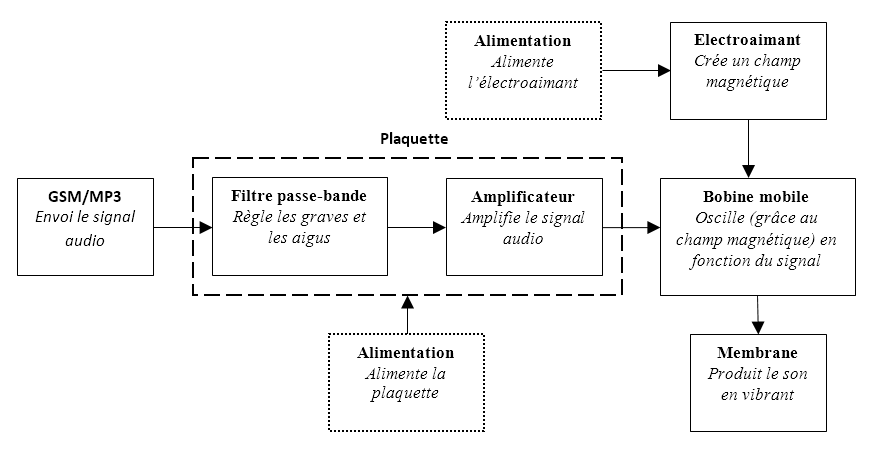
\includegraphics[scale=0.53]{schema_fonctionnel.png}
    \caption{Schéma fonctionnel du haut-parleur}
    \label{schema_fonctionnel}
\end{figure}
\end{frame}

% =======================================================================
%                   DIMENSIONNEMENT ELECTROAIMANT
% =======================================================================
\begin{frame}{Dimensionnement des bobines}

	\begin{columns}
		\begin{column}{5cm}
			\scalebox{0.2}{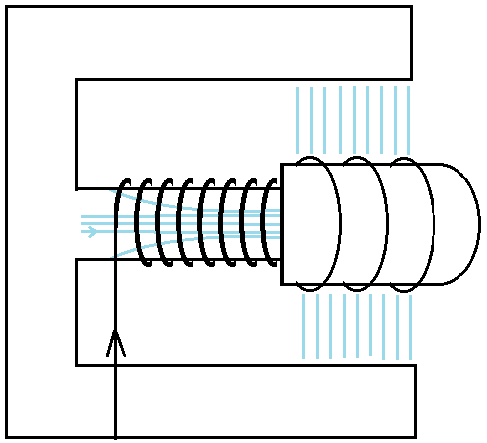
\includegraphics{hautparleur.png}}
		\end{column}

		\begin{column}{5cm}
			La bobine fixe joue un rôle d'électroaimant. Dans des conditions idéales, le champ total crée est $B = \unit{0.1143}{\tesla}$.
		\end{column}
	\end{columns}

	\bigbreak

	\paragraph{\textbf{Tableau récapitulatif}}
	\small
	{
		\begin{center}
		\begin{tabular}{c|c|c|c|c|c}
										& $N$ 	& $I$ 										& $R$ 								& $L$ 										& $L_{fil}$ \\
			\hline
			Bobine fixe 	& $400$ & \unit{2.5}{\ampere} 		& $7.254\Omega$ 	& \unit{0.01475}{\henry} 	& \unit{40.3}{\meter} \\
			\hline
			Bobine mobile & $118$ & \unit{0.1667}{\ampere}  & $2.38\Omega$ 	& \unit{0.0734}{\henry} 	& \unit{12.6}{\meter} \\
		\end{tabular}
		\end{center}
	}
\end{frame}

% =======================================================================
%                   DIMENSIONNEMENT DU HAUT-PARLEUR 
% =======================================================================
\begin{frame}{Dimensionnement du haut-parleur}
	\framesubtitle{Le boîtier}
		\begin{itemize}
			\item Cube de \unit{25}{\centi\meter} de côté ;
			\item Matériau MDF d'épaisseur \unit{18}{\milli\meter} ;
			\item Pieds en caoutchouc ;
			% Pieds en caoutchouc à rajouter!
			\item Porte coulissante à l'arrière.
		\end{itemize}

		% Ajouter une image ?
\end{frame}

\begin{frame}{Dimensionnement du haut-parleur}
	\framesubtitle{La membrane}
		\begin{itemize}
			\item Diamètre de \unit{17}{\centi\meter} ;
			\item Papier de densité \unit{200}{\gram\per\meter\squared}.
		\end{itemize}

		% Ajouter une image ?
\end{frame}

% =======================================================================
%                MODELISATION MECANIQUE DU HAUT-PARLEUR 
% =======================================================================
\begin{frame}{Modélisation mécanique du haut-parleur}
	\begin{figure}[ht]
		\minipage{0.4\textwidth}
			\underline{Équation du mouvement}
			$$m\fvdd{x}(t) = -k\fv{x}(t) + BLi(t)$$
			Hypothèses : 
				\begin{itemize}
					\item Négliger le poids de la bobine ;
					\item Négliger le frottement ;
				\end{itemize}
		\endminipage\hfill
		\minipage{0.4\textwidth}
			\underline{Observation importante}
			$$f = \frac{1}{2\pi} \cdot{\sqrt{\frac{k}{m}}}$$
			Fréquence de résonance, amplitude du mouvement infini.
		\endminipage\hfill
	\end{figure}
\end{frame}

% =======================================================================
%                				APPROXIMATION MATHEMATIQUE
% =======================================================================
\begin{frame}{Approximation mathématique}

	Fréquence de coupure : intersection entre la droite horizontale $y = 
	\unit{2.5}{\volt}$ et $y = a\log(x) + b$.

	\begin{figure}[ht!]
		\includegraphics[scale=0.6]{GRAPHE.png}
		\caption{Graphe expérimental de $V_{out}$ en fonction de la fréquence}
	\end{figure}
\end{frame}

\begin{frame}{Approximation mathématique}
	Système approché : 

	\begin{center}
		\begin{array}{rcel}
			$$
			\begin{pmatrix}
				4.204 & 1\\
				4.255 & 1 \\
				4.301 & 1
			\end{pmatrix} &

			\begin{pmatrix}
			a\\
			b
			\end{pmatrix} &

			= &

			\begin{pmatrix}
				1.607\\
				1.565\\
				1.524
			\end{pmatrix}
			$$
		\end{array}
	\end{center}

	$$\fbox{y = -1.96\log{x} + 9.84}$$

	$$\fbox{x = \unit{5557.7}{\hertz}}$$ 

	Fréquence théorique : $f = \frac{1}{2\pi RC} = \unit{5889.2}{\hertz}$ .

	Avec $R = \unit{57.5}{\ohm}$ et $C = \unit{470}{\nano\farad}$.
\end{frame}

% =======================================================================
%                							VALIDATION
% =======================================================================
% Il faut qu'on discute à propos de cette partie, est-ce qu'on la garde?
% C'est la partie la plus dangereuse car c'est celle qu'on maitrise le 
% moins.
\begin{frame}{Validation}
\begin{tabular}{cc}
	\includegraphics[scale=0.03]{P1010031.jpg} &  
	\includegraphics[scale=0.03]{P1010034.jpg} \\
	Sources de tension pour la plaquette & Test de la plaquette\\
	Sources + et - & Voir où est le problème\\
	& Données
\end{tabular}
\end{frame}

\begin{frame}
\begin{tabular}{cc}
   \includegraphics[scale=0.5]{Pmulti.jpg}& 
   \includegraphics[scale=0.15]{Ptesla.jpg} \\
	Resistance des bobines & Champ magnétique bobine\\
	Données pour dimentionnement& Champ suffisant\\
\end{tabular}
\end{frame}

% Valeurs à vérifier, j'ai quelques doutes
\begin{frame}{Compte-rendu}
	\begin{itemize}
		\item Tension des sources :  \unit{15}{\volt}
		\item Courant electroaimant : \unit{1}{\ampere}
		\item Resistance bobine fixe : \unit{2.38}{\ohm}
		\item Champ magnétique bobine fixe : \unit{0.08}{\tesla}
		\item Courant bobine fixe : \unit{0.116}{\ampere}
		\item IN : \unit{0.1}{\volt}
		\item OUT avec pentotiomètre : \unit{0.22}{\volt}
		\item OUT sans pentotiomètre : \unit{3}{\volt}
	\end{itemize}
\end{frame}

% =======================================================================
%                 							PLANNING 
% =======================================================================
% Partie peut-être superflue aussi, à discuter demain.
\begin{frame}{Le planning}

		\begin{tabular}{|c|c|c|}
		\hline
		Semaine & Théorique & Pratique \\
		\hline
		S2 & CdC &\\
		\hline
		S3 & Modélisation filtres &\\
		\hline
		S4 & Dim. électroaimant &\\
		\hline
		S5 & Recherches documentaires & \\
		\hline
		S6 & Préparation pré)jury & Bobinage + soudure\\
		\hline
		S7 & Pré rapport & Pré jury\\
		\hline
		S8 & & Test plaquette\\
		\hline
		S9-10 & & Membrane et caisson\\
		\hline
		S11-12 & Rédaction rapport & test son\\
		\hline
		S13-14 & Préparation défense orale &\\
		\hline

		\end{tabular}
\end{frame}

% =======================================================================
%                			MODELISATION DES FILTRES
% =======================================================================
\begin{frame}{Modélisation du filtre passe-haut}
	\begin{columns}
		\begin{column}{5cm}
			\scalebox{0.5}{\includegraphics{hgp_voltages.png}}
		\end{column}

		\begin{column}{5cm}
			\begin{itemize}
				\item $V_{out}$ est en retard de $\arctan{RC\omega}$ par rapport à $V_{in}$ ;
				\item Le déphasage augmente avec la fréquence.
			\end{itemize}
		\end{column}
	\end{columns}

	\begin{columns}
		\begin{column}{5cm}
			\begin{itemize}
				\item Atténue les basses fréquences ;
				\item Laisse passer les hautes fréquences.
			\end{itemize}
		\end{column}

		\begin{column}{5cm}
			\scalebox{0.5}
			{\includegraphics{hgp_ratio.png}}
		\end{column}
	\end{columns}
\end{frame}

% =======================================================================
\begin{frame}{Modélisation du filtre passe-bas}

	\begin{columns}
		\begin{column}{5cm}
			\scalebox{0.5}{\includegraphics{lwp_voltages.png}}
		\end{column}

		\begin{column}{5cm}
			\begin{itemize}
				\item $V_{out}$ est en retard de $\arctan{RC\omega}$ par rapport à $V_{in}$ ;
				\item Le déphasage augmente avec la fréquence.
			\end{itemize}
		\end{column}
	\end{columns}

	\begin{columns}
		\begin{column}{5cm}
			\begin{itemize}
				\item Atténue les hautes fréquences ;
				\item Laisse passer les basses fréquences.
			\end{itemize}
		\end{column}

		\begin{column}{5cm}
			\scalebox{0.5}{\includegraphics{lwp_ratio.png}}
		\end{column}
	\end{columns}
\end{frame}

% =======================================================================
%                			RECHERCHES DOCUMENTAIRES
% =======================================================================
\begin{frame}{Recherche documentaire}
	\framesubtitle{La contre-réaction (ou contre réaction négative)}

	\textbf{Principe} : réinjection d'une partie du signal de sortie à l'entrée.

	\begin{columns}
		\begin{column}{5cm}
			\includegraphics{opamp_loop.png}
		\end{column}

		\begin{column}{5cm}
				\begin{itemize}
					\item Signal de sortie plus proche du signal d'entrée ;
					\item	Réduction des signaux parasites et de la distorsion ;
					\item Contrôle du gain ;
					\item Elargissement de la bance passante ;
					\item Réduction de l'impédance de sortie.
				\end{itemize}
		\end{column}
	\end{columns}
\end{frame}

\begin{frame}{Recherche documentaire}
	\framesubtitle{La distorsion}

	\textbf{Principe} : des fréquences harmoniques s'ajoutent à la fréquence fondamentale
	$\Rightarrow$ modification du signal.

	\bigbreak

	\begin{columns}
		\begin{column}{5cm}
			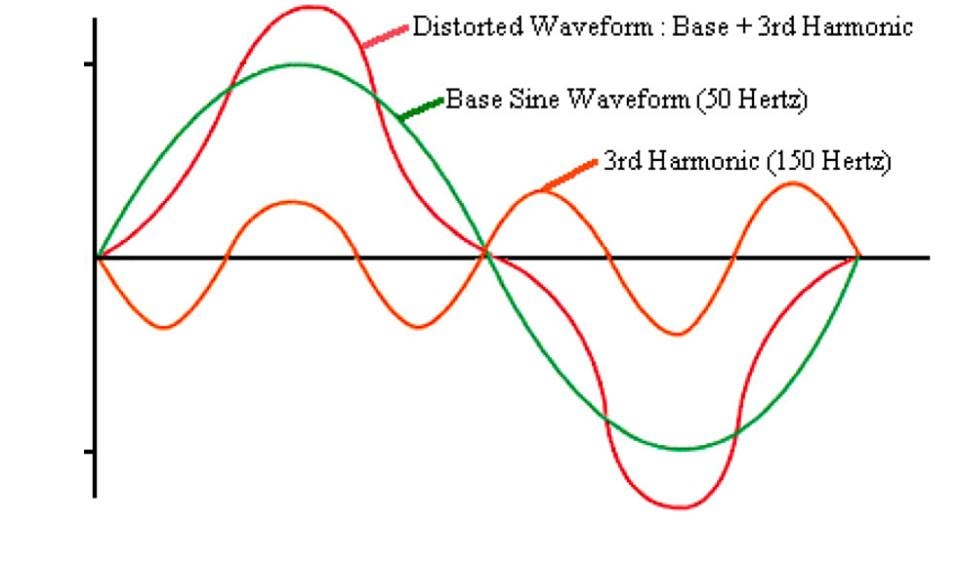
\includegraphics[scale=0.35]{distorsion.jpg}
		\end{column}

		\begin{column}{5cm}
			Conséquences :
			\begin{itemize}
				\item	Surchauffe des composants électroniques ;
			\end{itemize}

			Solutions :
			\begin{itemize}
				\item	Filtres actifs ou passifs (passe-haut et passe-bas) ;
				\item Boucle de contre-réaction (réduction du TDH de 1\% à 0.001\%).
			\end{itemize}
		\end{column}
	\end{columns}
\end{frame}
% =======================================================================
%                			CONCLUSION
% =======================================================================
\begin{frame}
 \frametitle{Conclusion}
 \begin{itemize}
		\item Nos erreurs;
		\item Nos apprentissages;
		\item Notre ressentit;
 \end{itemize}
\end{frame}

\end{document}
